\section{3DR Solo Dron}
Para este desarrollo se ha elegido el dron 3DR Solo distribuido por la empresa norteamericana \url{https://3dr.com/}. Este dron se encuentra en una gama alta debido a sus capacidades \url{https://3dr.com/solo-drone/specs/}, tales como batería, distancia de comunicacion y potencia, cualidades que lo hacen un dron muy versatil. Durante el desarrollo se ha usado la versión oficial del software de 3DR 2.4.2. Se eligió esa debido a que era una versión estable. A bordo de este dron se encuentra una placa estabilizadora Pixhawk 2.

\begin{figure}[H]
  \centering
  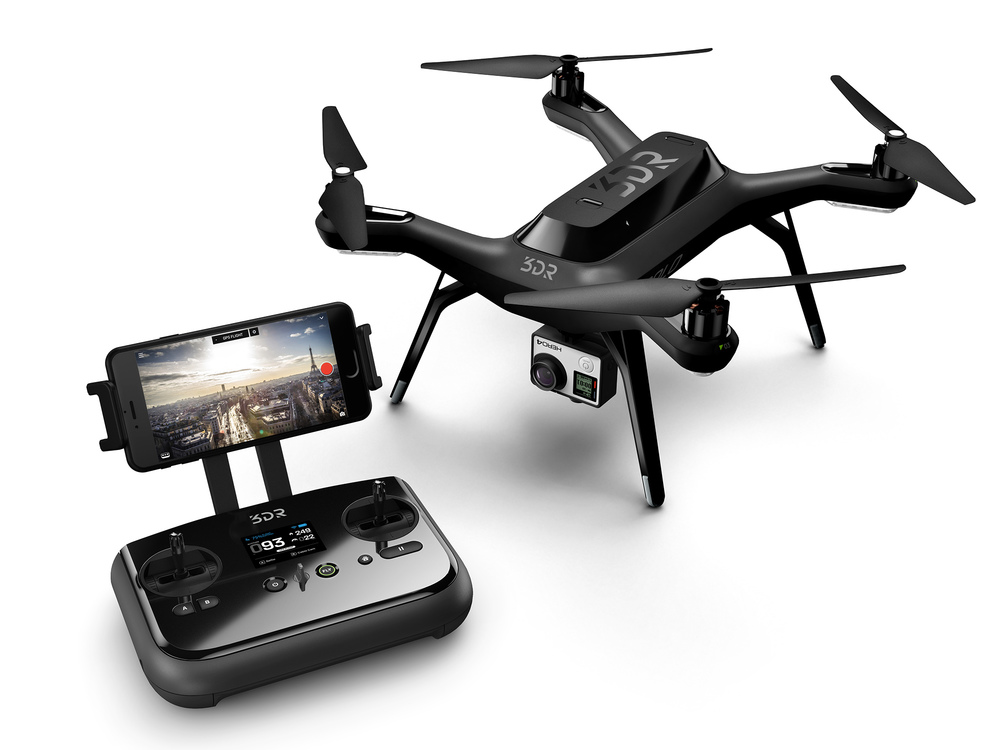
\includegraphics[scale=1]{imagenes/3drSoloDron.jpg}
  \caption{3DR Solo Drone}
  \label{fig:3drsolodrone}
\end{figure}


\cleardoublepage
\subsection{Placa estabilizadora Pixhawk}

Esta placa se trata de un desarrollo específico creado entre la "Pixhawk open hardware community" en colaboración con 3D Robotics y que vio como primer destinatario el 3DR Solo. Ofrece un interfaz que se apoya en comandos llamado MAVLink. A través de estos comandos se le puede también enviar órdenes al piloto automático quien las ejecutará más adelante trataremos el protocolo MAVLink en profundidad. El único modo de conectar con el 3DR Solo será a traves del mando, debido a que únicamente el mando es capaz de levantar la dirección IP a la que poder conectarse a ella. En posteriores evoluciones de la versión que controlan tanto el dron como el mando, desde los foros oficiales de 3DR \footnote{\url{https://3drpilots.com/threads/connecting-directly-to-the-pixhawk-2-on-a-solo.7926/}}, comentan que ya se aborda la solución de que sea el propio dron quien levante la dirección IP a la cual poder conectar y no tener que depender del enlace del mando.

La comunicación entre el driver y el dron quedaría de la siguiente forma:

\begin{figure}[H]
  \centering
  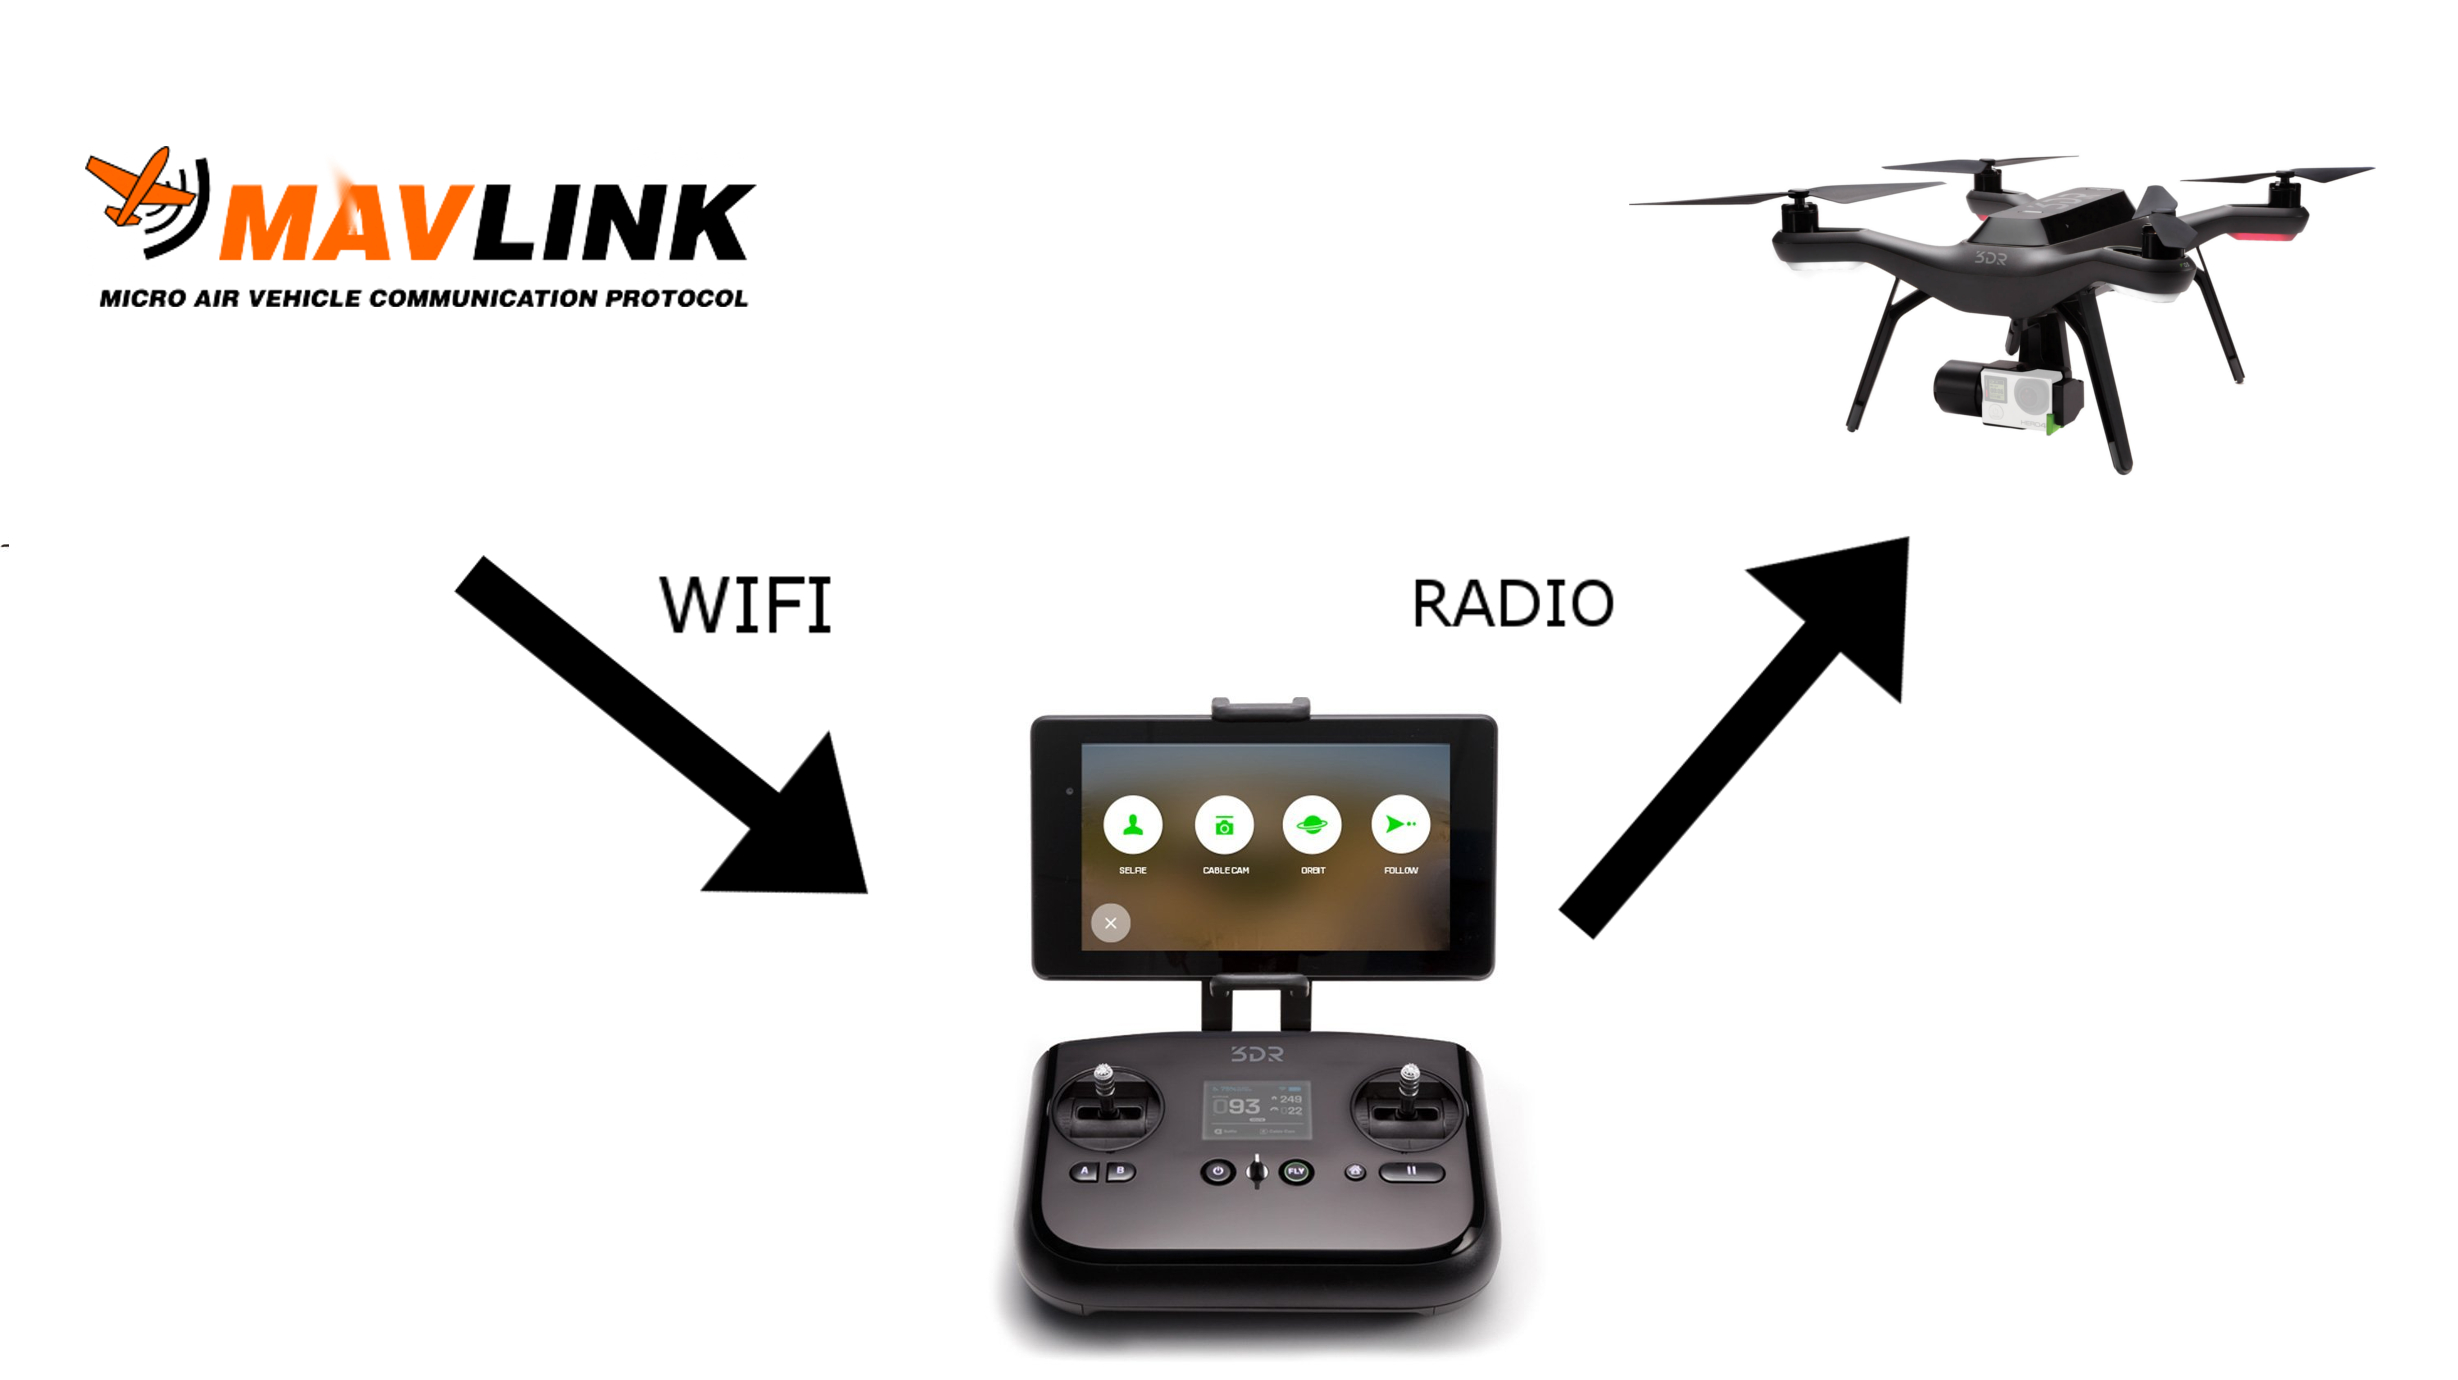
\includegraphics[scale=0.15]{imagenes/diagramaComunicacion.jpg}
  \caption{Diagrama comunicación}
  \label{fig:diagrama}
\end{figure}

\section{Protocolo MAVLink}
\label{sec:mavlink}

MAVLink siglas de Micro Air Vehicle Link es un protocolo de comunicación desarrollado para comunicar las placas estabilizadoras con piloto automático a los GCS o estación de tierra, las aplicaciones desde las que se podía enviar misiones y seguir el cumplimiento de las mismas desde tierra.
MAVLink se publicó\footnote{\url{https://github.com/mavlink/mavlink/commit/a087528b8146ddad17e9f39c1dd0c1353e5991d5}} en 2009 por Lorenz Meier, publicado bajo licencia LGPL aspira a convertirse en el protocolo standard en robótica aérea y se ha probado su funcionamiento en PX4, PIXHAWK, APM\footnote{Ardupilot Mega} y Parrot AR.Drone.

La versión actual que se está utilizando en este TFG es la 2.0.


La lista completa de los comandos se encuentra a en la pagina oficial de Mavlink\footnote{\url{http://mavlink.org/messages/common}}. Un ejemplo de los mensajes más importantes del protocolo y en el que se centra principalmente este TFG es el comando actuador de velocidad. Este comando hace uso de la estructura del mensaje "SET\_POSITION\_TARGET\_LOCAL\_NED", en el cual se indican las velocidades lineales que debe seguir en cada eje (velocidad medida en m/s). Este comando, en conjunto al actuador que hace uso de la rotación, cuya estructura es la del mensaje "COMMAND\_LONG", permite tener control total sobre el dron. 

Cada comando tiene un identificador único  el cual permite al dron reconocer la acción que se debe realizar. En función de este primer identificador los parámetros que se introducen a continuación permiten dar la información necesaria al dron para actuar. Esta comunicación y el contenido de los mensajes se comentará en mayor detalle en el apartado 4.1. Un ejemplo de la estructura del mensaje que se usa para GPS es el siguiente:
{\scriptsize
\begin{verbatim}
type GpsStatus struct {
    SatellitesVisible  uint8      Némero de satélites visibles
    SatellitePrn       [20]uint8  Id Global de cada satélite
    SatelliteUsed      [20]uint8  Lista con el uso de cada satélite
    SatelliteElevation [20]uint8  Elevación, nos da el ángulo sobre el horizonte.
    SatelliteAzimuth   [20]uint8  Dirección del satélite, 0: 0 grados, 255: 360 grados.
    SatelliteSnr       [20]uint8  Señal/ruido de cada uno de los satélites
}
\end{verbatim}}
Este mensaje trae la informacin del enlace actual con el GPS y se envía periódicamente en ciclos que decidimos en parámetros de conexión con el dispositivo.

En la figura \ref{fig:comunicacionMavLink} se puede comprobar que en la estructura de comunicación que se realiza entre la estación de tierra y cada componente se establece una conexión, en la cual continuamente se intercambian mensajes con información, ya sea para comunicar una acción, reclamar el estado de algún componente interno, como podría ser la batería, o un simple ACK para mantener la conexión activa, este último mensaje también es usado en este TFG para comprobar que la conexión con el dron sigue activa desde cualquier componente.


\begin{figure}[H]
  \centering
  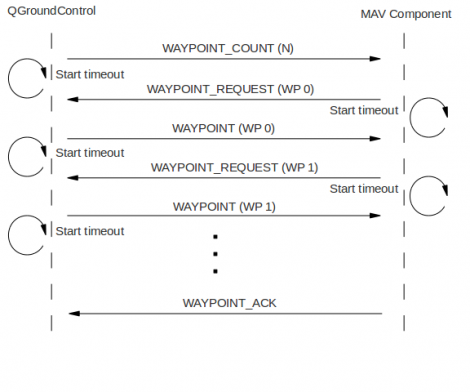
\includegraphics[scale=0.5]{imagenes/comunicacionMavLink.png}
  \caption{Comunicación MavLink}
  \label{fig:comunicacionMavLink}
\end{figure}

\section{JdeRobot}
\label{sec:jderobot}

JdeRobot es un entorno desarrollado por el laboratorio de robótica de la Universidad Rey Juan Carlos, para el desarrollo de aplicaciones de robótica. Su última realease la 5.6 se liberó el 9 de Octubre de 2017 pudiendo ver los detalles de ésta en el github oficial\footnote{\url{https://github.com/JdeRobot/JdeRobot/wiki/JdeRobot-5.6.0}}.
JdeRobot se compone de interfaces, drivers, utilidades y aplicaciones para el desarrollo de cualquier proyecto de robótica, se apoya en estos interfaces, algunos de ellos los veremos en profundidad a continuación, para interconectar entre sí todos los aplicativos del mismo y en Zeroc ICE para la comunicaci\'on entre ellos.
Algunos de los drivers más importantes que contiene:
\begin{enumerate}
\item Cameraserver. Se trata de un driver para enviar imágenes y video a través del interfaz camera
\item Gazeboserver. Driver desarrollado para conectar los robots en el simulador Gazebo con aplicaciones y así poder simular los desarrollos \footnote{\url{http://jderobot.org/Daniyague-pfc}}.
\item Ardrone\_server. Driver que conecta el Parrot Ar-Drone a JdeRobot\footnote{\url{http://jderobot.org/Amartinflorido-tfg}}. Este driver escrito en c++ transforma el conjunto de comandos AT del drone en interfaces y viceversa, implementa los interfaces camera, cmdvel, navdata, extra y pose3D y permite acceder a la actitud del drone así como a sus 2 cámaras. Sirve también datos como el nivel de la batería y permite grabar vídeo o tomar fotos.
\end{enumerate}
Algunas de las herramientas web desarrolladas más importantes serían:
\begin{enumerate}
\item Cameraview. Se trata de una aplicaci\'on desarrollada en c++ capaz de recibir vídeo a través del interfaz camera.
\item UAV viewer. Aplicaci\'on desarrollada como ground control de robots aéreos. Esta aplicaci\'on permite teleoperar cualquier tipo de robot aéreo y ofrece de forma visualmente atractiva datos como la actitud, velocidades lineales y angulares, ofrece también la posibilidad de visualizar videos servidos por el interfaz camera. \footnote{\url{http://jderobot.org/Amartinflorido-tfg}}.
\end{enumerate}
En este TFG se ha abordado la creacion de un nuevo driver y la versión mejorada de una herramienta de visualización y manejo de drones.

\section{Interfaces relativos a los drones}
JdeRobot dispone de más de 30 interfaces pero en este cap\'itulo se explica lo que se han utilizado durante el desarrollo:
\begin{itemize}
\item Pose3D. Utilizado para recoger los datos de actitud y la posici\'on de la aeronave.
{\scriptsize
\begin{verbatim}
Pose3DData
  {
	float x;  /* x coord */
	float y;  /* y coord */
	float z;  /* z coord */
  	float h;  /* */
	float q0; /* qw */
	float q1; /* qx */
	float q2; /* qy */
	float q3; /* qz */
  };
\end{verbatim}}
\item CMDVel. Utilizado para enviar comandos de velocidad.
{\scriptsize
\begin{verbatim}
	class CMDVelData
	{
		float linearX;
		float linearY;
		float linearZ;
		float angularX;
		float angularY;
		float angularZ;										
	};

\end{verbatim}}
\item Extra. Utilizado principalmente para las \'ordenes de despegue y aterrizaje.
{\scriptsize
\begin{verbatim}
    void land() - land drone. 
    void takeoff() - takeoff drone. 
    void reset() 
    void recordOnUsb(bool record) 
    void ledAnimation(int type,float duration, float req) 
    void flightAnimation(int type, float duration) 
    void flatTrim() 
    void toggleCam() - switch camera. 
\end{verbatim}}

\end{itemize}

\section{ICE}
\label{sec:ICE}
ICE (Internet Communications Engine) es un \textit{middleware}  orientado a objetos que proporciona llamadas a procedimientos remotos, \textit{grid computing} y funcionalidad cliente / servidor desarrollada por ZeroC bajo GNU GPL y una licencia privativa. Está disponible para C ++,
Java, .Net languages, Objective-C, Python, PHP y Ruby, en la mayoría de los sistemas operativos. También hay una versión para teléfonos móviles llamada Ice-e. ICE permite desarrollar aplicaciones distribuidas con un esfuerzo mínimo, abstraer al programador para que interactúe con una red baja interfaces de trabajo. El proceso de desarrollo de aplicaciones debe enfocarse solo en la lógica y no en las peculiaridades de la red. Es un \textit{middleware} multilenguaje y así, podemos implementar clientes y servidores en diferentes lenguajes de programación y en diferentes plataformas. ICE trabaja con objetos distribuidos, de modo que dos objetos en nuestra aplicación no necesita ejecutarse en la misma máquina. Los objetos pueden estar en diferentes máquinas y comunicarse a través de la red a través del envío de mensajes entre ellos.

JdeRobot utiliza ICE para la comunicación entre sus nodos, por lo tanto, la tarea de leer
los valores de un sensor u órdenes de comando a un robot son tan simples como ejecutar un método de un objeto en la aplicación. Una ventaja significativa es la posibilidad de desarrollar aplicaciones independientes del contexto. Un programador puede desarrollar un controlador en C ++ para un robot particular que está incrustado en el robot, por otro lado, otro desarrollador puede desarrollar una aplicación para el procesamiento de imágenes en Python que se ejecuta en una PC. Mediante ICE podemos usar estas dos aplicaciones, que originalmente eran independientes, como un solo aplicación sin tener que preocuparse por las comunicaciones de bajo nivel. Con esto podemos desarrollar aplicaciones modulares de gran complejidad sin esfuerzo adicional.

La conexión entre el driver y las aplicaciones de control, como la prpia herraiente de teleoperacion, se realiza usando este middleware.

\section{Python}
\label{sec:python}

Python es un lenguaje de programaci\'on interpretado y multiplataforma que naci\'o en los años 80 en los país bajos con idea de hacer más legible el c\'odigo.
El lenguaje de programaci\'on que inicialmente se utilizaba principalmente para scripting, ha sabido crecer con los años y con la publicaci\'on de Python3 en 2009 ha recibido el impulso que necesitaba para ser hoy en día el 5º lenguaje mas utilizado por encima de PHP, .NET y Javascript que baja hasta el 8º puesto según TIOBE en un estudio de Abril de 2017.

El porqué de utilizar Python, muy sencillo mantiene el carácter multiplataforma de JdeRobot, su c\'odigo es simple y legible y trabaja muy bien con dependencias muy utilizadas en rob\'otica como OpenCV.

Tanto el driver como la herramienta desarrolladas en este TFG se han creado empleando Python 2.7. Esta decisión se debe a que JdeRobot es compatible con ROS y éste \textit{framework} únicamente es compatible en dicha versión de Python. Actualmente se encuentra preparada una versión en el repositorio migrado a la versión de Python 3.5.

\cleardoublepage